\documentclass[10pt,a4paper]{article}
\usepackage[a4paper,margin=14mm]{geometry}
\usepackage{graphicx}
\usepackage{booktabs}
\usepackage{amsmath}
\usepackage{microtype}
\usepackage[compact]{titlesec}
\usepackage[font=small,labelfont=bf,skip=4pt]{caption}
\usepackage[round,authoryear]{natbib}
\usepackage{xcolor}
\usepackage[hidelinks]{hyperref}

\renewcommand{\topfraction}{0.95}
\renewcommand{\bottomfraction}{0.9}
\renewcommand{\textfraction}{0.05}
\renewcommand{\floatpagefraction}{0.9}
\setcounter{topnumber}{3}
\setcounter{totalnumber}{5}
\setlength{\bibsep}{2.5pt}
\setlength{\floatsep}{7pt plus 2pt minus 2pt}
\setlength{\textfloatsep}{9pt plus 2pt minus 4pt}

\newcommand{\tbf}[1]{\textbf{#1}}
\newcommand{\todo}[1]{\textcolor{red}{[TODO: #1]}}

\title{\vspace{-8mm}Lesion-mask supervision for rejecting unseen plant diseases:\\a controlled comparison on PlantSeg}
\author{\todo{student name(s) and ID(s)}}
\date{AIP304 Machine Learning, Coursework 2 (Option 2: research challenge)}

\begin{document}
\maketitle
\vspace{-6mm}

\section{Problem, motivation, and hypothesis}
A plant-disease classifier deployed in the field will meet host--disease combinations that were absent
from its training data. A practical system should therefore name the diseases it knows and decline the
ones it does not. This report studies the Option~2 question: does adding binary lesion-mask supervision
during training improve rejection of held-out disease classes on familiar hosts over a matched classifier
trained without it, while maintaining known-class macro-F1? Every prediction uses only the RGB image.

The hypothesis was recorded in writing before formal training (protocol of 2026-11-11). Support requires,
in each of the two class assignments: (i) mean familiar-host AUOSCR improves by at least 0.02 over the
matched baseline, (ii) at least 2 of 3 paired seeds improve, and (iii) mean known-class macro-F1 falls by
no more than 0.02. Any other pattern counts as non-support, and small or seed-inconsistent differences
are reported as descriptive observations only.

\section{Related work}
Unknown plant-disease recognition is an established area \citep{dong2024impact}, and three settings should
be kept apart. Rejecting an unknown class, the setting studied here, asks the model to withhold a label.
Identifying an unseen class asks it to predict a combination never seen in training, as in the
self-supervised approach of \citet{chai2024beyond}. Abstaining on healthy images is a third behaviour,
addressed for grounded agricultural recognition by \citet{alshehhi2026agroground}. Our study concerns only
the first setting.

The closest method is PAG-MSBNet \citep{yan2026pag}, which pursues lesion-focused open-set crop-disease
recognition through prototype-aware gated multi-scale branches. Its supervision, architecture, data, and
evaluation protocol all differ from ours. It engineers lesion-guided features inside a purpose-built
network, whereas we ask whether a plain auxiliary binary-segmentation loss changes the open-set behaviour
of a standard classifier. \citet{dong2024impact} compare fine-tuning paradigms for unknown plant-disease
recognition but do not isolate binary mask supervision under a matched training budget. We found no prior
study that isolates this single factor under controlled backbone, budget, and hyperparameter search, so
this investigation is a new controlled comparison rather than a replication.

Rejection is scored from the classifier itself. We evaluate maximum softmax probability
\citep{hendrycks2017baseline}, maximum logit, and negative energy \citep{liu2020energy}; \citet{vaze2022openset}
argue that closed-set quality largely determines such open-set performance. Our primary metric, AUOSCR,
follows \citet{dhamija2018reducing}.

\section{Data and protocol}
We use PlantSeg~v7 \citep{wei2025plantseg,wei2026plantseg}, restricted to the nine coursework hosts:
4{,}349 images across 43 host--disease classes. Two audits preceded modelling. A pixel-hash duplicate
check after EXIF orientation correction found 73 cross-partition duplicate groups, 34 with conflicting
labels; conflicting groups were removed entirely, remaining duplicates deduplicated (201 images
excluded). A near-duplicate screen (brightness correlation, perceptual and difference hashes, mirrored
and cropped variants) yielded 436 candidate pairs, 213 confirmed by visual inspection; the same rule
excluded a further 209 images. The retained set has 3{,}939 images in the original approximately
70/10/20 partitions. Cross-partition leakage was the audit's target; heavy crops or rotations could still
evade it, which we note as a limitation.

Class roles follow the task sheet. Citrus is the development-unfamiliar control and potato the
test-unfamiliar control. For each remaining host, disease labels are sorted alphabetically;
Assignment~A reserves the first category as development unknown and the second as test unknown,
Assignment~B the second and third. Each assignment keeps 25 known classes; known training classes
have 18--134 images each, so both arms train under the same imbalance (the partition-composition figure
is in the notebook). Frozen manifests (SHA-256 recorded) fix image identifiers, roles, and partitions for
both arms. Assignment~A uses 1{,}576 known training images; validation has 266 known, 54 familiar-host
unknown, and 39 citrus images; test has 490 known, 137 familiar-host unknown, and 26 potato images.
Assignment~B uses 1{,}432 training; 246/64/39 validation; 452/132/26 test. Training images of reserved
classes were discarded, development unknowns were used for validation only, and no test-unknown image
entered training, feature fitting, calibration, or selection.

\section{Method}
\subsection{Matched training arms}
Both arms use an ImageNet-pretrained ResNet-18 \citep{he2016deep} with a 25-way classification head,
trained from the generic pretrained initialisation. Images are EXIF-transposed, resized aspect-preserving
to a 224-px long side, padded with the ImageNet mean, and normalised with the pretrained statistics.
Augmentation is horizontal flips plus mild brightness and contrast jitter (0.1); augmented copies stay
with their original training image, and evaluation transforms are deterministic. Both arms use AdamW
\citep{loshchilov2019decoupled}, batch size 32, 20 epochs, cosine decay to $10^{-6}$, weight decay
$10^{-4}$, and the same learning-rate candidates $\{10^{-4}, 3\times10^{-4}\}$.

The lesion arm adds one component: a lightweight binary segmentation head at \texttt{layer2}
(U-Net style; \citealp{ronneberger2015unet}), supervised by the known-class lesion masks. Its loss is the
mean of binary cross-entropy and soft Dice \citep{milletari2016vnet}, weighted by 0.25 and added to the
classification cross-entropy; padded regions are excluded. Validation and test predictions never use
masks: the mask branch is discarded at inference.

The mechanism under test is representational. If the shared trunk must localise symptom pixels, its
features may become more disease-specific and less tied to host or background appearance. That shift could
separate unseen diseases on known hosts from the known classes in score space. The mechanism can also
fail for a plain reason: features that discriminate known diseases need not rank unfamiliar ones, and
better localisation may mainly sharpen known-class boundaries.

\subsection{Scores, thresholds, and freezing}
All three scores are computed from the same trained network: MSP \citep{hendrycks2017baseline}, MaxLogit,
and negative energy \citep{liu2020energy}. The primary rule was selected on baseline validation runs
only: MaxLogit had the highest mean familiar-host validation AUOSCR (0.627 over 12 baseline runs, versus
0.624 for negative energy and 0.623 for MSP) and was then applied to both arms. Learning rates were
selected per assignment under the pre-registered rule: both candidates satisfied the macro-F1 tolerance
(mean paired known-validation macro-F1 differences of $+0.0028$ at $10^{-4}$ and $-0.0100$ at
$3\times10^{-4}$), and $10^{-4}$ maximised mean familiar-host validation AUOSCR in both assignments.
Checkpoints were chosen by maximum known-validation macro-F1 (earliest epoch on ties); selected epochs
ranged from 7 to 19, and the learning curves are in the notebook. Each model and seed received its own
threshold, set to the largest known-validation score accepting at least 95\% of known validation images
(observed calibration acceptance 95.11--95.12\%). All choices for both assignments, including weights and
thresholds, were frozen in a checksummed file before any test inference.

\section{Experiments and results}
Table~\ref{tab:main} reports the frozen test results: means and standard deviations over three paired
seeds, per assignment and arm.

\begin{table}[t]
\centering
\caption{Frozen MaxLogit test results, mean $\pm$ SD over 3 paired seeds. AUOSCR, unknown false
acceptance (FA), and AUROC refer to familiar-host unknowns; the last column is the unfamiliar-host
(potato) control. Paired differences (lesion $-$ baseline) follow the $\pm$ sign.}
\label{tab:main}
\small
\begin{tabular}{llccccc}
\toprule
 & Arm & Familiar AUOSCR & Known macro-F1 & Known acc. & FA rate & Unfam.\ AUOSCR \\
\midrule
A & Baseline & 0.6245 $\pm$ 0.0115 & 0.7578 $\pm$ 0.0203 & 0.7850 $\pm$ 0.0123 & 0.825 $\pm$ 0.044 & 0.6385 $\pm$ 0.023 \\
A & Lesion   & 0.6316 $\pm$ 0.0048 & 0.7589 $\pm$ 0.0095 & 0.7844 $\pm$ 0.0042 & 0.830 $\pm$ 0.053 & 0.6441 $\pm$ 0.025 \\
B & Baseline & 0.6007 $\pm$ 0.0119 & 0.7017 $\pm$ 0.0099 & 0.7471 $\pm$ 0.0092 & 0.753 $\pm$ 0.052 & 0.6386 $\pm$ 0.007 \\
B & Lesion   & 0.5987 $\pm$ 0.0141 & 0.7031 $\pm$ 0.0065 & 0.7478 $\pm$ 0.0080 & 0.765 $\pm$ 0.042 & 0.6426 $\pm$ 0.007 \\
\bottomrule
\end{tabular}
\end{table}

\subsection{Primary outcome}
The pre-registered criterion was not met in either assignment
(Figure~\ref{fig:paired}). Mean familiar-host AUOSCR improved by $+0.0071$ in Assignment~A with 2 of 3
seeds positive, and fell by $-0.0020$ in Assignment~B with 1 of 3 positive. Neither difference approaches
the required $+0.02$, and the seed-level pairing is inconsistent. Under the criteria fixed before
training, the evidence does not support the hypothesis that lesion supervision improves rejection of
unfamiliar diseases on familiar hosts. Known-class performance was preserved as required: macro-F1
differences were $+0.0011$ (A) and $+0.0014$ (B), well inside the 0.02 tolerance, and the same holds for
accuracy. The OSCR curves of the two arms nearly coincide in both assignments
(Figure~\ref{fig:oscr}), which is the curve-level view of the same result.

\begin{figure}[t]
\centering
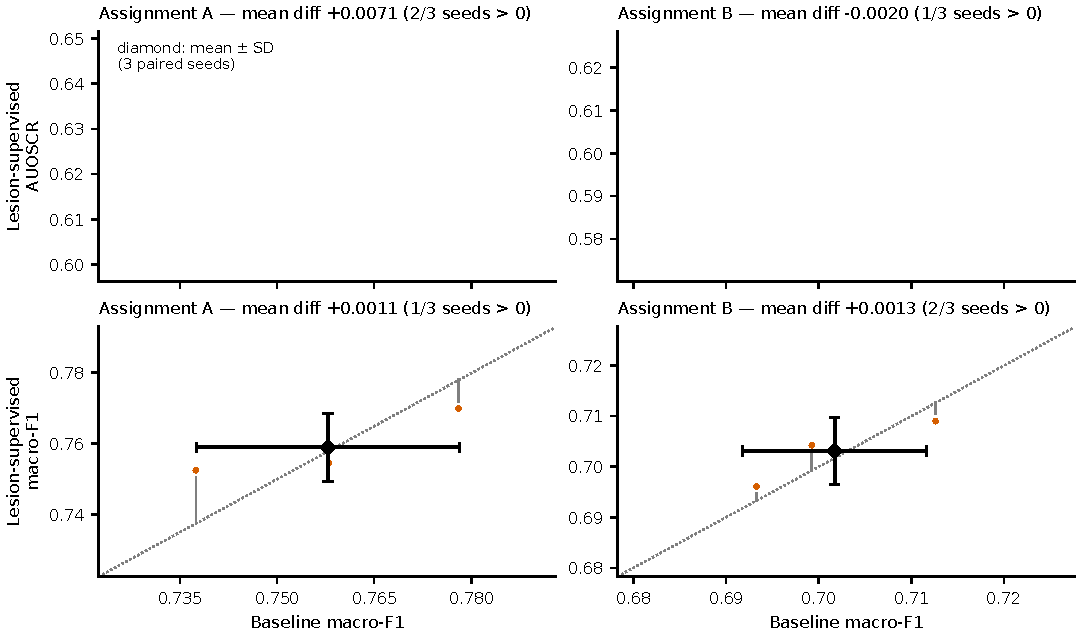
\includegraphics[width=0.82\linewidth]{figures/fig3_paired_seeds.pdf}
\caption{Paired seed-level comparison (3 seeds). Each point pairs one seed's baseline value (x) with the
lesion-supervised value (y); grey drops connect pairs to the identity line; the black diamond is the seed
mean $\pm$ SD. Top row: familiar-host AUOSCR (A $+0.0071$, 2/3 seeds $>0$; B $-0.0020$, 1/3). Bottom row:
known-class macro-F1 (A $+0.0011$, B $+0.0014$). Differences are descriptive; no significance test was
pre-registered.}
\label{fig:paired}
\end{figure}

\begin{figure}[t]
\centering
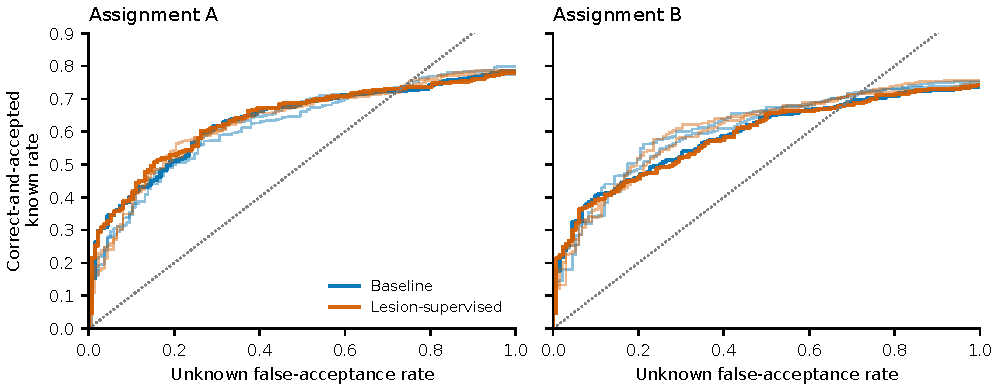
\includegraphics[width=0.88\linewidth]{figures/fig5_oscr_curves.pdf}
\caption{Open-set classification-rate curves: correct-and-accepted known rate against familiar-host
unknown false-acceptance rate, swept over all thresholds, per seed (thick line: seed 42; thin: seeds 123
and 2026; blue: baseline, vermillion: lesion-supervised). Seed means of the areas under these curves are
the AUOSCR values in Table~\ref{tab:main}; the near-coincidence of the two arms' curves matches the small
paired differences.}
\label{fig:oscr}
\end{figure}

\subsection{Operating point and error structure}
At the frozen thresholds, test known acceptance stayed near 91--93\% and the correct-and-accepted known
rate near 0.72--0.76 (A: 0.757 baseline, 0.757 lesion; B: 0.715, 0.721), while most familiar-host
unknowns were still accepted: false-acceptance rates averaged 82.5\% (baseline) and 83.0\% (lesion) in
Assignment~A, and 75.3\% and 76.5\% in Assignment~B. Figure~\ref{fig:scores} shows why. The MaxLogit
distributions of known and familiar-host unknown images overlap heavily, and the validation-calibrated
thresholds fall inside the unknown mode, so no threshold near this operating point separates the groups.

The accepted unknowns are not random (Figure~\ref{fig:dest}). The most frequent confusions pair visually
similar diseases on the same host, such as zucchini powdery mildew accepted as zucchini yellow mosaic
virus, and wheat leaf rust as wheat stripe rust. In Assignment~B the dominant flow is apple rust
(a test-unknown class) accepted as apple scab. Known-class errors follow the same within-host pattern
(Figure~\ref{fig:conf}): of the pooled seed-level judgments, 91.5\% and 91.4\% (A, baseline and lesion)
and 90.1\% and 90.6\% (B) stay on the true host, and 60--63\% of the class-level errors are within-host
disease confusions (A: 191/316 and 190/317; B: 209/343 and 214/342). The largest single off-diagonal cell
in every matrix is tomato yellow leaf curl virus confused with tomato mosaic virus (13--17 judgments). In
validation diagnostics, corn northern-leaf-blight images (a familiar-host unknown in B) were accepted in
24 of 27 seed-level judgments by lesion-supervised models, 18 of them as gray leaf spot. The confusion is
systematic rather than seed-specific. The full 25$\times$25 class-level matrices and all four host-level
panels are in the notebook.

Splitting familiar-host unknowns by whether their disease name also occurs among known classes on another
host showed no consistent advantage for either arm (A: shared 0.639 vs.\ 0.637, unseen 0.622 vs.\ 0.631
for baseline vs.\ lesion; B: shared 0.589 vs.\ 0.586, unseen 0.615 vs.\ 0.614), although the groups are
unbalanced (A: 18 shared and 119 unseen images; B: 72 and 60). The unfamiliar-host (potato) control is
reported separately in Table~\ref{tab:main}; we make no claims about unfamiliar hosts generally, since the
protocol provides only potato. Per-image examples (notebook gallery) show the failure is image-specific
rather than class-uniform: in Assignment~A the highest-scoring false accept is an apple mosaic virus image
accepted as soybean mosaic (median MaxLogit 9.6, a shared disease name), while in Assignment~B apple rust
images span both the lowest-scoring correct reject (2.1) and false accepts as apple scab (7.4--7.6).

\begin{figure}[t]
\centering
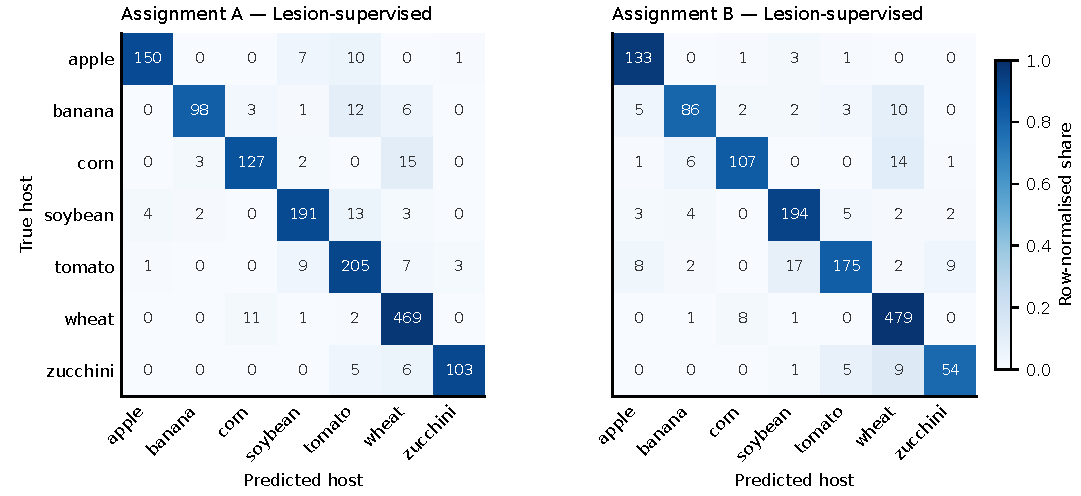
\includegraphics[width=\linewidth]{figures/fig7_host_confusion_report.pdf}
\caption{Known-class test confusion aggregated to the seven familiar hosts, pooled over the three
lesion-supervised seeds (cell numbers are seed-level judgments; A: 1{,}470, B: 1{,}356). The mass sits on
the diagonal (91.4\% of A and 90.6\% of B judgments stay on the true host), and most off-diagonal
class-level errors are within-host disease confusions (A: 190/316, B: 214/342); the largest single cell is
tomato yellow leaf curl virus confused with tomato mosaic virus. Baseline panels are nearly identical; the
full 25$\times$25 class-level matrices and all four host-level panels are in the notebook.}
\label{fig:conf}
\end{figure}

\begin{figure}[t]
\centering
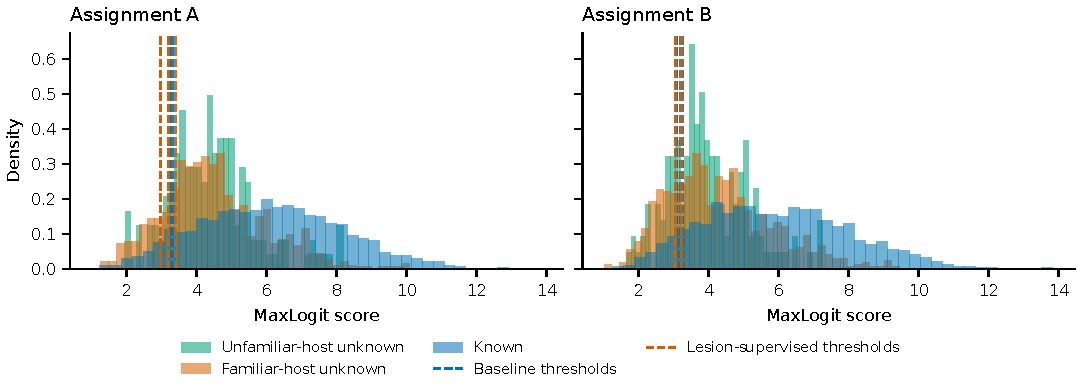
\includegraphics[width=0.97\linewidth]{figures/fig2_score_distributions.pdf}
\caption{Test MaxLogit score distributions pooled over the six models per assignment (baseline and lesion
$\times$ 3 seeds), for known, familiar-host unknown, and unfamiliar-host unknown images. Dashed lines are
the per-model, per-seed thresholds calibrated on known validation images to accept at least 95\% of them.
A: $n=490/137/26$; B: $n=452/132/26$. The distributions overlap heavily and the thresholds fall inside the
familiar-host unknown mode.}
\label{fig:scores}
\end{figure}

\begin{figure}[t]
\centering
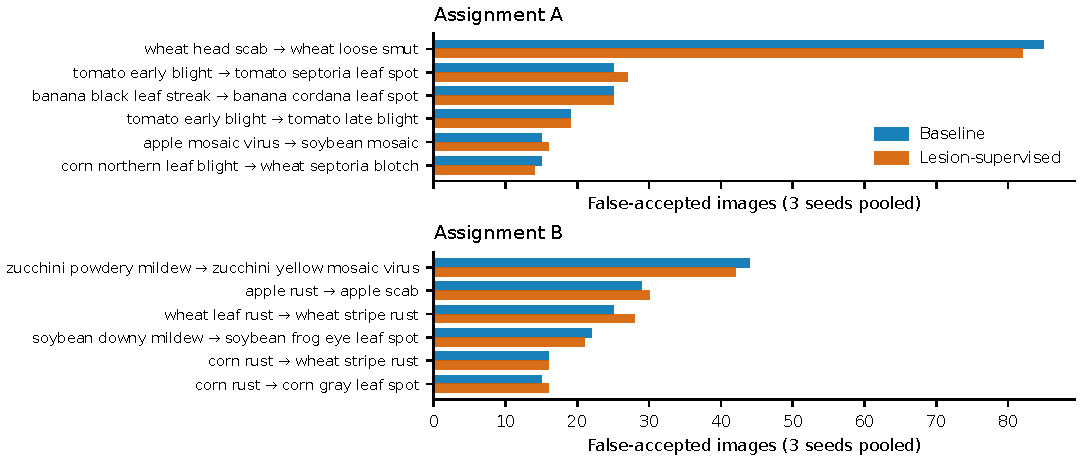
\includegraphics[width=\linewidth]{figures/fig4_false_acceptance_destinations_top6.pdf}
\caption{The six most frequent true-unknown to predicted-known destinations for familiar-host test
unknowns accepted at the frozen thresholds, pooled over 3 seeds per arm (A: 137 unknown images, 411
seed-level judgments per arm; B: 132, 396). The dominant confusions pair visually similar diseases on the
same host; the full top-ten ranking and a per-image prediction gallery are in the notebook.}
\label{fig:dest}
\end{figure}

\section{Interpretation and limitations}
The direct answer to the coursework question is no, under the pre-registered criteria: lesion-mask
supervision preserved known-class recognition but did not measurably improve rejection of held-out
diseases on familiar hosts. Assignment~A moved slightly positive and Assignment~B slightly negative, and
neither approached the 0.02 gain the hypothesis required. The mechanism failure is visible in
Figure~\ref{fig:scores}: with these features, familiar-host unknowns simply score like known images. In
qualitative validation diagnostics (notebook), the lesion branch's pixel heatmaps did highlight visible
symptoms, including on untrained diseases, so symptom localisation was partly achieved; it did not
translate into more selective open-set scores. This pattern is consistent with the observation of
\citet{vaze2022openset} that open-set behaviour tracks closed-set quality, which barely changed here.

Several limits bound this conclusion. The lesion-loss weight (0.25) and head placement were fixed by the
protocol and not ablated, and the shuffled-mask control suggested by the task sheet was not run, so we
cannot exclude that a different weighting behaves differently. Three paired seeds give descriptive
statistics only; no significance test was pre-registered. One backbone and optimiser were used, so the
result does not attribute the shortfall to ResNet-18 or AdamW specifically. The near-duplicate audit
covered cross-partition pairs and inspected crops and rotations only within its candidate set. The
unfamiliar-host control contains only potato, and the fixed 95\% operating point was inherited from the
protocol rather than chosen for this data. Within these limits, the comparison remains fair: both arms
shared initialisation, augmentation, budget, and search, and every configuration was frozen before test
inference.

\section{AI-use disclosure and contributions}
\todo{single author or team contribution statement: name each member's work on implementation,
experiments, analysis, writing, and demonstration, or state single-author completion.}
AI tools were used with the author remaining responsible for correctness, originality, citations, and
reproducibility. An OpenAI Codex CLI agent assisted with data-audit scripting, experiment design, and
notebook implementation. A GitHub Copilot agent (VS Code, November 2026 sessions) assisted with figure
redesign, including a programmatic readability audit, and with drafting this report. The project's
academic-humanizer and scientific-visualization procedure guides were applied in prose editing and figure
quality checks. Outputs were verified by the checks the notebook records: dataset ZIP MD5, manifest and
checkpoint SHA-256 checksums, independent recomputation of all reported metrics from the per-image
prediction files (912 comparisons, maximum absolute deviation $7.8\times10^{-16}$), frozen configuration
files, and local execution on Apple MPS (Python 3.12, PyTorch 2.8.0, torchvision 0.23.0; the 24-run grid
took approximately 3.7 hours). Training followed the PyTorch transfer-learning workflow
\citep{chilamkurthy2025transfer}.

\bibliographystyle{plainnat}
{\footnotesize\bibliography{refs}}

\end{document}
